\chapter{Análisis del Sistema} 

\section{Comparación de Cosas }

Estado del arte  del sistema

Las partes más importantes de cada módulo que compone el sistema, como el porque se usaron ciertos componentes eléctricos o la raspberry o el linux en la raspberry.  

\section{Requerimientos funcionales.}
\begin{itemize}
    \item Mecanismo de generación de energía eléctrica.
    \begin{itemize}
        \item Medir el voltaje y corriente que está generando la celda solar.
        \item Medir la temperatura de la batería.
        \item Medir la corriente que produce la batería.
        \item Regular la carga y descarga de la batería.
        \item Por medio de un sistema mecánico colocar la celda solar en la inclinación  que le sea la más perpendicular a los rayos del sol
    \end{itemize}
\end{itemize}

\begin{itemize}
    \item Interfaz de comunicación
    \begin{itemize}
     \item Transmitir el valor de los parámetros eléctricos (voltaje, corriente, temperatura, ángulo de posicionamiento) que se miden en el mecanismo de generación de energía eléctrica. 
    \end{itemize}
\end{itemize}

\begin{itemize}
    \item Aplicación móvil
    \begin{itemize}
     \item Indicar los dispositivos  en los que se puede usar la energía almacenada en la batería, para energizar dichos dispositivos .
     \item Mostrar gráficos que indiquen el rendimiento que  tiene el mecanismo de generación de energía eléctrica.
     \item Mostrar noticias e información acerca de las energías renovables.
     \item Permitir crear una cuenta a los usuarios.
     \item Permitir ingresar los datos personales de cada usuario.
     \item Panel de información que permita ser un punto de acceso a las diversas funciones que tiene la aplicación.
    \end{itemize}
\end{itemize}

\section{Requerimientos no funcionales.}

\begin{itemize}
    \item Mostrar mensajes de error que sean informativos y orientados al usuario final.
    \item La aplicación móvil debe ser compatible con la versión de Android xxx.xx
    \item Tener manuales de usuario del sistema estructurados adecuadamente.
    \item Girar el panel solar en dos ejes.
    \item Alimentar el sistema mecánico con la energía generada por el mismo sistema.
    \item La aplicación móvil debe poseer un diseño responsivo a fin de garantizar la correcta visualización en los diferentes dispositivos móviles.
    \item Mostrar los datos censados del mecanismo de generación de energía en el mismo mecanismo. 
\end{itemize}


\section{Diagrama de proceso.}

A continuación se muestra el diagrama que modela el proceso y funcionamiento que debe de tener el sistema, en él se detallan los módulos y usuarios que están presentes, asimismo el como interactúan entre ellos.

\begin{figure}[H]
\centering
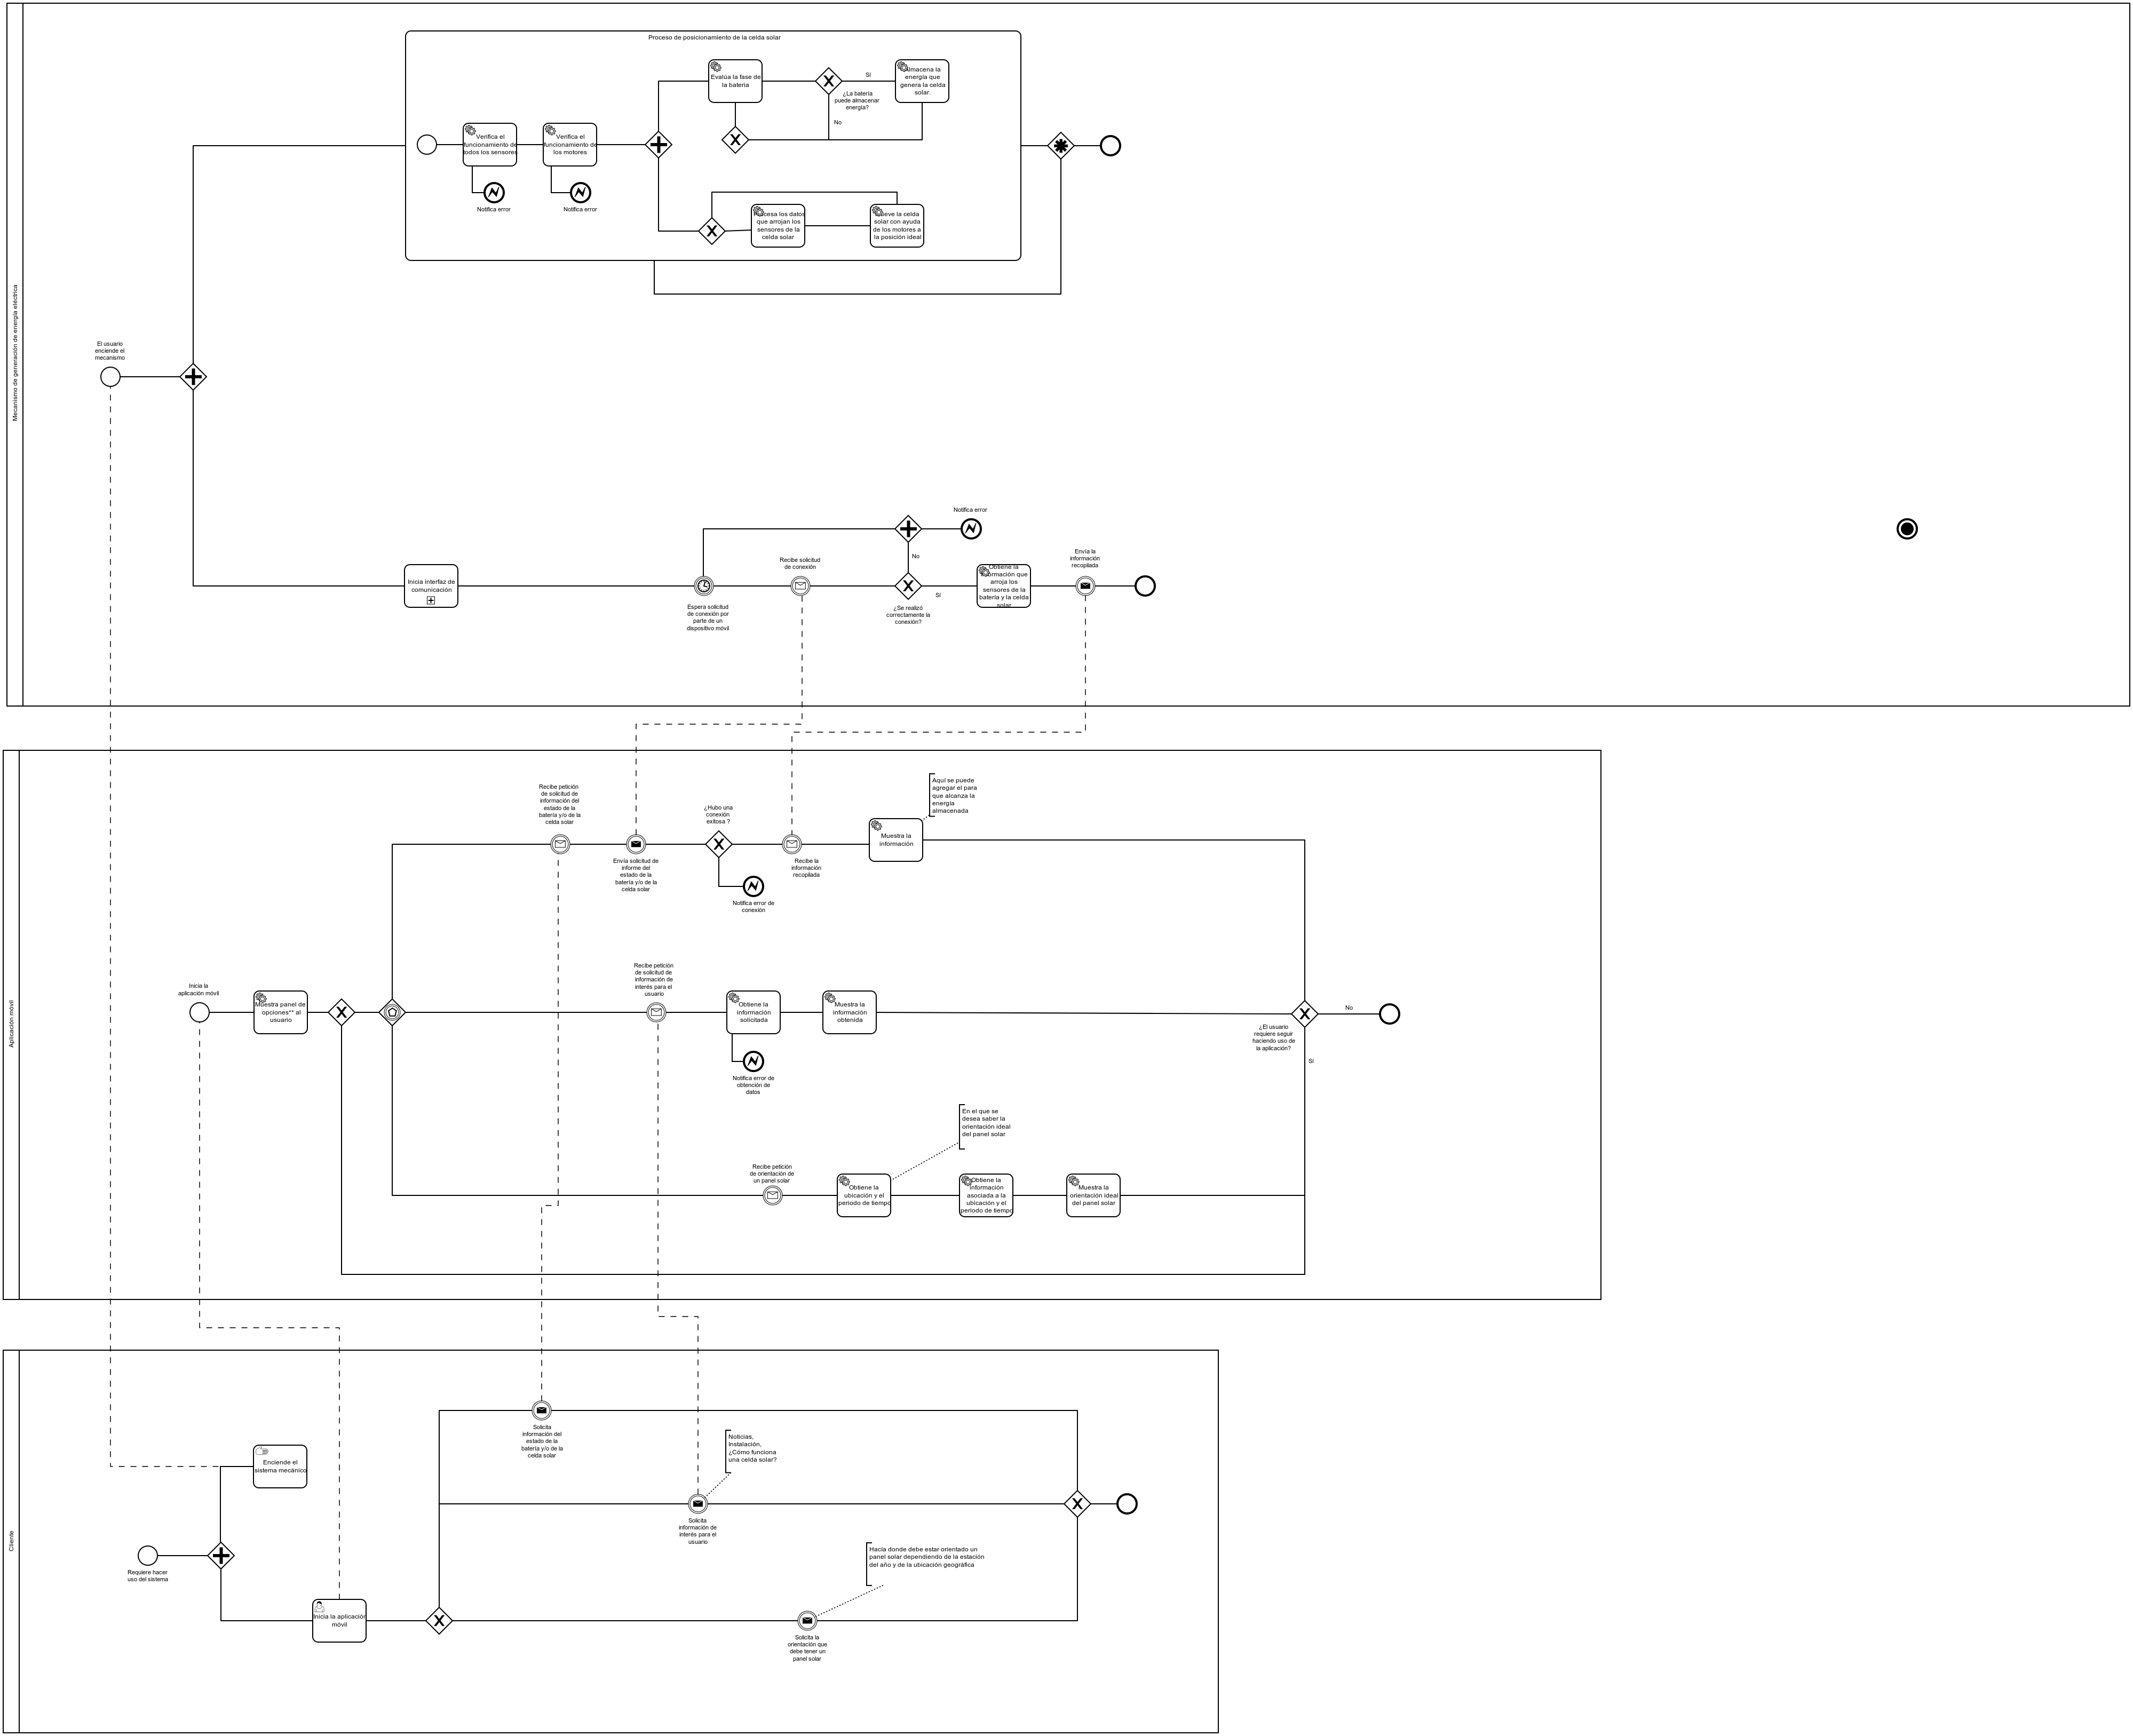
\includegraphics[width=23cm, height=17cm, angle=90]{./images/analisis/proceso.png}
\caption{Proceso del sistema}
\label{fig:1-1-1}
\end{figure}





